\documentclass[12pt]{article}

\usepackage{sbc-template}
\usepackage{graphicx,url}
\usepackage[utf8]{inputenc}

%\usepackage[brazil]{babel}
%\usepackage[latin1]{inputenc}

\sloppy

\title{Relações Binárias em Conjuntos\\Trabalho Prático de Matemática Discreta}

\author{André Taiar\inst{1}}


\address{Departamento de Ciência da Computação -- Universidade Federal de Minas
Gerais (UFMG)\\
  \email{taiar@dcc.ufmg.br}
}

\begin{document}

\maketitle

\begin{resumo}
  Na matemática e na lógica, uma relação binária é uma relação qualquer entre
  dois elementos (um conjunto de pares ordenados). As relações binárias são comuns
  em muitas áreas da ciência para definir muitas propriedades e conceitos. Neste
  trabalho, foram analisados arquivos que mapeavam diversos conjuntos e as
  relações entre seus elementos e essas foram classificadas de acordo com as
  suas propriedades.
\end{resumo}


\section{Relações em grafos} %mudar esse título

Em matemática e ciência da computação, grafo é o objeto básico de estudo da
teoria dos grafos. Tipicamente, um grafo é representado como um conjunto de
pontos (vértices) ligados por retas (as arestas).

\begin{figure}[ht]
\centering
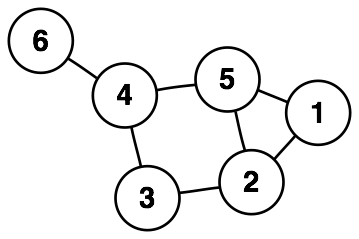
\includegraphics[width=.5\textwidth]{grafoEx.png}
\caption{Exemplo ilustrativo de um grafo com 6 vértices e 7 arestas}
\label{fig:exampleFig1}
\end{figure}

Utilizei neste trabalho um grafo para representar a relação entre os elementos
que foram passados na entrada. Cada elemento é representado como um vértice do
grafo e, se um elemento tem relação com outro elemento qualquer, eles são ligados
por uma aresta.

Para facilitar a análise das relações através do grafo, este foi implementado
utilizando uma matriz de adjacência como veremos no detalhamento das estruturas de
dados.

\section{Estruturas de dados e implementações}

O programa foi desenvolvido em 4 módulos: o módulo principal que cuida da leitura
do arquivo de entrada, da geração da saída e da lógica do funcionamento do programa
em si, o módulo que contém a implementação do grafo por matriz de adjacência, um
módulo com a implementação de uma lista encadeada utilizada em diversas partes
do programa e um módulo com a implementação da análise das relações utilizando o grafo.

\subsection{Implementação do grafo}

\subsubsection{Matriz de adjacência}

Vamos supor um conjunto com os seguintes elementos: $A = {1,2,3,4,5}$

Vamos dispor esses elementos numa tabela da seguinte forma:

\begin{center}
\begin{tabular}{llllll}
* & \textbf{1} & \textbf{2} & \textbf{3} & \textbf{4} & \textbf{5}\\
\textbf{1} & 0 & 0 & 0 & 0 & 0\\
\textbf{2} & 0 & 0 & 0 & 0 & 0\\
\textbf{3} & 0 & 0 & 0 & 0 & 0\\
\textbf{4} & 0 & 0 & 0 & 0 & 0\\
\textbf{5} & 0 & 0 & 0 & 0 & 0
\end{tabular}
\end{center}

Em nossa implementação, se temos dois elementos relacionados, marcamos as célula em 
comum dos dois elementos com o valor 1. Por exemplo, vamos relacionar os elementos da 
seguinte forma:

$\forall x \in A, (x, x) \in R$

Na matriz ficaria:

\begin{center}
\begin{tabular}{llllll}
* & \textbf{1} & \textbf{2} & \textbf{3} & \textbf{4} & \textbf{5}\\
\textbf{1} & 1 & 0 & 0 & 0 & 0\\
\textbf{2} & 0 & 1 & 0 & 0 & 0\\
\textbf{3} & 0 & 0 & 1 & 0 & 0\\
\textbf{4} & 0 & 0 & 0 & 1 & 0\\
\textbf{5} & 0 & 0 & 0 & 0 & 1
\end{tabular}
\end{center}

\subsection{Lista encadeada}

As listas encadeadas foram utilizadas no programa para armazenar pares ordenados dos 
elementos dos conjuntos que inicialmente não temos idéia de quantos serão.
Por exemplo: ao analisar os pares que faltam para completar um fecho transitivo, 
como não temos certeza da quantidade de pares que irão faltar, utilizamos uma
lista encadeada, que é uma estrutura de dados dinâmica (pois trabalha com alocação 
dinâmica de memória) para armazenar quantos pares quisermos e, ao final, fazer
a listagem de todos eles.

\subsection{Análise das relações}

Com o grafo implementado como uma matriz de adjacência, verificar as relações entre 
os elementos foram operações simples e pouco custosas (se resumem a trabalhar
com os índices correspondentes aos elementos e avaliar se o valor da célula da aresta 
correspondente estava ligada ou desligada). Não tenho certeza se trabalhei
com os melhores algoritmos para as avaliações mas eles estão funcionando corretamente 
para todos os testes que efetuei.

\subsubsection{Reflexiva}
Para avaliar se a relação é \textbf{reflexiva} bastou verificar se toda a
diagonal principal da matriz tinha o valor 1 o que significa que todos os
elementos são relacionados si próprios.

\subsubsection{Irreflexiva}
Para avaliar se a relação é \textbf{irreflexiva} bastou verificar se toda a
diagonal principal da matriz tinha o valor 0 o que significa que nenhum dos
elementos é relacionado com si próprio.

\subsubsection{Simétrica}
Para avaliar se a relação é \textbf{simétrica}, verifiquei se a matriz era
simétrica em relação à diagonal principal, ou seja: se a posição
$[i,j]$ da matriz estava relacionada com a posição $[j,i]$.

\subsubsection{Anti-Simétrica}
Para avaliar se a relação é \textbf{anti-simétrica}, procurei por pares tais que
$[i,j] = [j,i]$. Caso encontrasse algum, comparava se $i = j$. Caso verdadeiro,
para todos os pares, a relação é dita anti-simétrica.

\subsubsection{Assimétrica}
Para avaliar se a relação é \textbf{assimétrica}, verifiquei se a matriz não
tinha simetria com relação à diagonal principal, ou seja, verificar se todas as
posições $[i,j]$ eram diferentes das posições $[j,i]$.

\subsubsection{Transitiva}
Para avaliar se a relação é \textbf{transitiva}, verifiquei para todas as
posições $[i,j]$ se existia uma posição $[j,k]$ válida. Caso sim, verificava se
a posição $[i,k]$ também era válida. Caso isso acontecesse para todas
permutações de $i, j, k$ válidas, a relação é dita transitiva.

\subsubsection{Fecho Transitivo}
Para avaliar o \textbf{fecho transitivo} da relação

\end{document}
